\scanpage{82}
\mspage{81}
\uline{NB} Ceci détermine $P$ et l'application $A\longrightarrow|A|$ à iso can près.
\margin{Je présume que les conditions $(\mathrm{i}_{\unsure{M|\mu}})$ $(\unsure{\mathrm{ii}'_M|\mathrm{iii}'_M|\mathrm{iii}_M})$ $(\mathrm{iv}_M)$, $(\mathrm{v}_M)$ (ou $\mathrm{At\ L\,2}$) seront satisfaites automatiquement...}

Je pense notamment, en dehors du cas des \unsure{Antos|Autos} quasi-ensemblistes, au cas où on part d'un espace topologique $P$, et où on définit $\unsure{L|\mathcal{L}}$ \inserted{(``lieux'')} comme l'ens des parties compactes contractiles \inserted{de $P$} disons.

\margin{$\unsure{\uparrow|1}$}
On construit des ``quasi-simplexes'' de tte dimension \inserted{\unsure{arbitraire}} (ou de dimension \unsure{comb.|cohom.} majorée, p. ex. par $1$) par des conditions ad hoc, généralisant celles qui définissent une \unsure{fameuse} ficelle. [Dans le cas de $\dim\leq1$, j'ai \unsure{eu|bien} une définition en forme \unsure{ds|dans} l'esprit]. On définit $|X|$ de façon évidente. Tout marche ! Mais on fera attention que si on se borne aux lieux qui se trouvent sur une ficelle donnée, et à la fonction support ci dessus, la condition $\mathrm{Supp}_P^2$ n'est plus satisfaite en général.

% slanted
\margin{Attention, ici la fonction $X\longmapsto|X|$ ne satisfait pas $\mathrm{Supp}_P^1$.}
\uline{Exemple} Je prends la ``ficelle à deux brins''
\figure{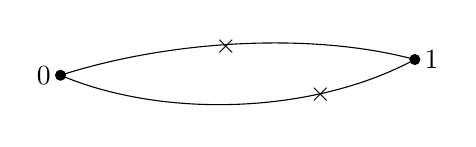
\begin{tikzpicture}[x=1cm,y=1cm]
\draw (0,0) .. controls (1.4,.45) and (3.2,.55) .. (4.5,.2);
\draw (0,0) .. controls (1.3,-.55) and (3.2,-.5) .. (4.5,.2);
\fill (0,0) circle (2pt) node[left] {$0$};
\fill (4.5,.2) circle (2pt) node[right] {$1$};
\node at (2.1,.37) {$\times$};
\node at (3.3,-.24) {$\times$};
\end{tikzpicture}}
dont les lieux \inserted{(en dehors de $0,1$)} \unsure{seront les|sont les} ``sections'' \inserted{\unsure{fermées}} de l'un et l'autre brin -- ils s'identifient donc \deleted{aux} aux éléments de l'ens ordonné produit
\[
I^{\circ}=\mathopen{]}0,1\mathclose{[}\times\mathopen{]}0,1\mathclose{[}.
\]
